\section{INSTRUMENTOS}\label{ins}
El conjunto de instrumentos se elabor\'o con los  siguientes recursos:
\begin{itemize}
\item Humanos
	\begin{itemize}
	\item Profesionales -i.e. Entrenadores-.
	\item Atletas
	\item Investigador
	\end{itemize}
\item No humanos
	\begin{itemize}
	\item Mesa de soporte, con una altura de 0.70 metros.
	\item Cable de extensi\'on el\'ectrico de 2.00 metros. 
	\item Computadora p\'ortatil
		\begin{itemize}
		\item Conector de carga de alimentaci\'on
		\end{itemize}
	\item Sensor Kinect
		\begin{itemize}
		\item Adaptador del Kinect
		\end{itemize}
	\end{itemize}
\end{itemize}
\subsection{Formulario de registro de movimiento} \label{ins:frmMov}
Este formulario se adjunta en anexos (ver figura \ref{fig:frmWhiteMov}), la cual tiene como objetivo describir el movimiento de cada equipo deportivo. Por otra parte, el formulario esta compuesto por las siguientes incisos:
\begin{itemize}
	\item \textbf{Nombre del movimiento:} Nombre que se identifica en gu\'ias deportivas o de salud.
	\item \textbf{Descripci\'on del movimiento: } Contesta la pregunta: ?`Qu\'e es el movimiento?
	\item \textbf{Movimiento unilateral:} S\'i es afirmativo, el movimiento trabaja con solo una parte del cuerpo (Izquierda o derecha, ejemplo una patada), en caso contrario el movimiento trabajo con todas las partes del cuerpo (Izquierda y derecha, ejemplo un salto).
	\item \textbf{Partes del cuerpo ignorada:} M\'ultiples respuestas, que identifica las articulaciones ignoradas -i.e. Debido que no es informaci\'on relevante para el movimiento-:
	\begin{itemize}
		\item \textbf{Brazo derecho o izquierdo:} Ignora las siguientes articulaciones (seg\'un su lado):Pulgar, dedo del medio, mano, codo, hombro, centro de los hombros, cuello, cabeza y espalda.
		\item \textbf{Cuerpo inferior:} Ignora las siguientes articulaciones (en ambos lados): centro de cadera, caderas, Rodillas, Tobillos y p\'ies.
	\end{itemize}
		\item \textbf{N\'umero de pasos:} Cantidad de pasos del movimiento.
		\item \textbf{Offset del paso:} Cantidad que identifica la etiqueta del movimiento.
		\item \textbf{Valor de identificaci\'on:} Describe el valor del rango general de un paso.
		\item \textbf{Detalle por paso:} Es  importante conocer:
			\begin{itemize}
		\item \textbf{Paso:} N\'umero \'unico que identifica el paso.
		\item \textbf{Diagrama:} Imagen visual del paso -i.e. Seguimiento de esqueleto-.
		\item \textbf{Descripci\'on del paso:} Responde la pregunta: ?`Cu\'al es la postura del cuerpo durante ese paso?
		\item \textbf{Etiqueta:} N\'umero \'unico que identifica el paso a partir de la probabilidad de movimiento.
	\item \textbf{Rango de identificaci\'on:} Rango m\'aximo que identifica el paso dentro de la probabilidad del movimiento.
	\end{itemize}
\end{itemize}
\subsection{Formulario de registro de rutina} \label{ins:frmRout}
Formulario adjuntado en anexos (Ver figura \ref{fig:frmWhiteRout}), que tiene como funci\'on identificar los ejercicios de calentamiento  previamente a realizar el movimiento seleccionado por cada equipo deportivo, adem\'as de estandarizar el n\'umero de repeticiones del movimiento por cada atleta, a partir de los siguientes puntos:
\begin{itemize}
	\item \textbf{Descripci\'on del calentamiento:} Detalla el tipo de calentamiento -e.g. Calentamiento con tu propio peso, calentamiento dentro de un ambiente, calentamiento a partir de objetos-.
	\item \textbf{Movimientos:} Enlista los movimientos que se realiza durante el calentamiento (Validado por las unidades de an\'alisis, secci\'on  \ref{sj:ua}).
	\item \textbf{Series:} Cantidad de veces que debe realizar un atleta, un conjunto de repeticiones del movimiento.
	\item \textbf{Repeticiones:} Cantidad de repeticiones del movimiento.
	\item \textbf{Tiempo:} duraci\'on del calentamiento.
	\item \textbf{Im\'agenes:} Fotograf\'ias tomadas durante el entrenamiento de cada equipo deportivo.
	\item \textbf{Nombre del movimiento:} Movimiento seleccionado por cada equipo deportivo  (secci\'on  \ref{ins:frmMov}).
	\item \textbf{Rutina:} Describe el tipo de rutina para la captura de datos:
	\begin{itemize}
		\item \textbf{For time:} M\'axima cantidad de repeticiones del movimiento, durante un tiempo establecido.
		\item \textbf{Escaleras:} N\'umeros de repeticiones establecida, separada por series.
	\end{itemize}	
\end{itemize}
\subsection{Interfaces de usuarios} \label{ins:UI}
Aplicaciones que interact\'ua con el usuario para la recoleccio\'n de datos, en donde se trabaja con  tres tipos:
\subsubsection{Presentation Foundation (WPF)}
\label{ins:UI:wpf}
El desarrollador, \citeA{wpf2019}, menciona que este tipo de interfaz permite crear aplicaciones de escritorio con el framework .NET, la cual es soportado desde Windows XP hasta la \'ultima versi\'on de Windows -i.e. Windows 10-. Por lo tanto, en el presente proyecto se utiliz\'o este tipo de interfaz para la construci\'on del seguimiento de esqueleto, generada por los siguientes Kit de desarrollo de software:
\begin{itemize}
	\item \textbf{Windows inputs} Herramienta que permite crear elementos de un formulario -e.g. Botones, checkbox, textbox-.
	\item \textbf{Windows Media} Herramientas que permite renderizar el seguimiento de esqueleto en tiempo real a partir de pinceles, colores, formas y dibujos.
	\item \textbf{Windows Threading} Herramientas que permite crear temporizadores -i.e timer- para la renderizaci\'on del seguimiento del esqueleto en un per\'iodo del tiempo -i.e. 30 fps-.
	\item \textbf{Kinect} Herramientas que permite acceder a las funcionalidades del Kinect, tales:
	\begin{itemize}
	\item \textbf{Sensor Kinect:} Accede al API del Kinect para realizar las siguientes tareas:
		\begin{itemize}
				\item \textbf{Body frame reader:} Obtiene la informaci\'on del seguimiento del esqueleto -i.e. Esqueletos reconocidos con sus respectivas articulaciones-.
				\item \textbf{Estado del sensor:} Activo, Pausa, No detectado e inactivo.
				\item \textbf{Datos del visual Gesture Builder:} Normalizaci\'on de datos del sensor del Kinect para el uso del modelo de machine learning.
		\end{itemize}	
			\item \textbf{Joint type:} Enumeradores que enlista las articulaciones del seguimiento del esqueleto -e.g. Manos, codos, hombros-.
			\item \textbf{Visualizaci\'on de los recursos de los frames para Visual Gesture Builder:} Interpreta la base de datos de gesturas y posiciones de un movimiento.
	\end{itemize}	 
\end{itemize}
A partir de los kits de desarrollo, se cre\'o 2 aplicaciones para la captura de informaci\'on.
\paragraph{Detecci\'on de profundidad}\mbox{} \\ \label{ins:UI:wpf:depth}
Esta aplicaci\'on tiene como objetivo recolectar la distancia correcta de profundidad entre el atleta y el Kinect, tomando en cuenta una articulaci\'on de an\'alisis, adem\'as de la altura del usuario medida desde la cabeza hasta los p\'ies, tal como se presenta en la siguiente imagen:
\begin{figure}[H]
	\caption{Interfaz gr\'afica de detecci\'on de profundidad entre el usuario y el sensor}
	\label{fig:appDepth}
	\centering
	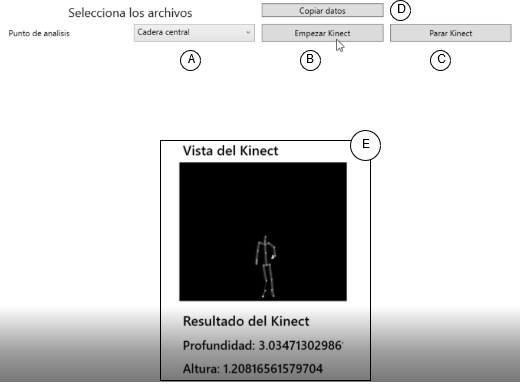
\includegraphics[width=380px,height=200px]{graphics/appProfundidad.png} \\
	\textbf{Fuente:} Aplicaci\'on elaborada por el autor de tesis
\end{figure}
Esta interfaz se compone por 5 componentes:
\begin{enumerate}[A.]
    \item Combo box que permite seleccionar la articulaci\'on de an\'alisis.
    \item Bot\'on que empieza las funcionalidades del seguimiento del esqueleto.
    \item Bot\'on que finaliza las funcionalidades del seguimiento del esqueleto.
    \item Conjunto de paneles de control, que muestra una imagen en tiempo real del seguimiento del esqueleto, adem\'as de la altura (en metros) del usuario y la distancia de profundidad (en metros) entre el atleta y el sensor.
        \item Bot\'on que permite copiar a una hoja de observaci\'on (ver anexos, cuadro \ref{tab:obsDepth}) los siguientes datos respectivos: N\'umero de identificaci\'on de la articulaci\'on, la distancia de profundidad y la altura del usuario.
\end{enumerate}
\paragraph{Evaluaci\'on del movimiento}\mbox{} \\\label{ins:UI:wpf:evaluate}
Aplicaci\'on realizada por el autor del usuario, cuya funcionalidad es programar una rutina de tabata a partir de del movimiento de cada equipo deportivo, mostrado en la siguiente imagen:
\begin{figure}[H]
	\caption{Interfaz gr\'afica de evaluaci\'on de un movimiento}
	\label{fig:appEvaluate}
	\centering
	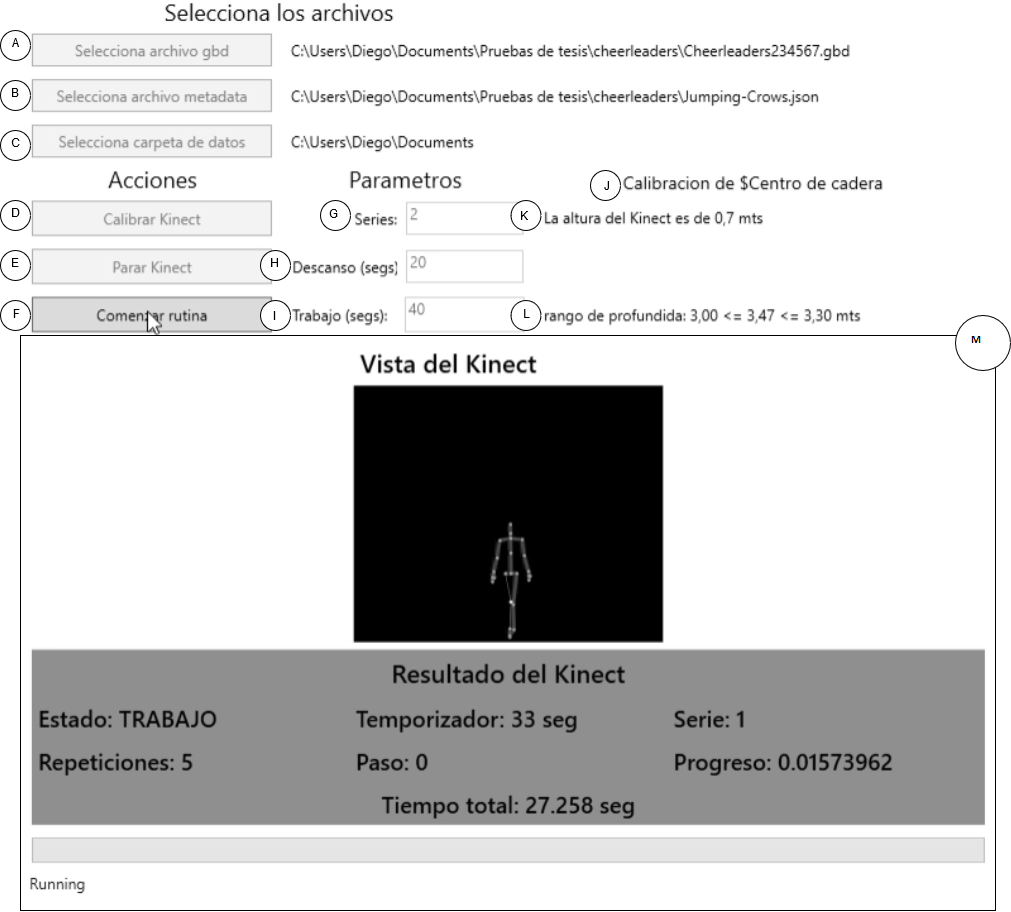
\includegraphics[width=380px,height=250px]{graphics/appEvaluacion.png} \\
	\textbf{Fuente:} Aplicaci\'on elaborada por el autor de tesis
\end{figure}
Interfaz que se divide en 13 componentes:
\begin{enumerate}[A.]
    \item Bot\'on que permite seleccionar el archivo de base de datos del reconocimiento del movimiento.
    \item Bot\'on que permite seleccionar el archivo json que contiene toda la informaci\'on respectiva del movimiento (ver anexos, c\'odigo  \ref{code:jsonMeta}).
    \item Bot\'on que permite seleccionar la direcci\'on del archivo de resultado de tabata.
    \item Bot\'on que permite activar todas las funcionalidades del Kinect.    
    \item Bot\'on que permite detener todas las funcionalidades del Kinect. 
    \item Bot\'on que permite comenzar la rutina de tabata (en tiempo real).
   \item  Text box n\'umerico que indica la cantidad de tiempos de trabajo y descanso del atleta durante su rutina de tabata.
   \item  Text box n\'umerico que se\~nala el tiempo de descanso durante su rutina.
   \item  Text box n\'umerico que muestra el tiempo de trabajo durante su rutina -i.e. Durante este tiempo, el atleta debe realizar la cantidad m\'axima de repeticiones-.
   \item  Etiqueta de articulaci\'on de \'analisis para medir la distancia de profundidad entre el atleta y el sensor.
   \item  Etiqueta de la altura  recomendada (en metros)  del sensor y el suelo.
      \item  Etiqueta de la distancia m\'inima y m\'axima de profundidad del atleta con respecto al sensor, y por otra parte indica la distancia profundidad actual del usuario y el sensor.
      \item Conjunto de paneles de controles que muestra:
      \begin{itemize}
            \item  El seguimiento de esqueleto en tiempo real.
            \item  Estado actual de la rutina: Inicio, Trabajo, Descanso, Fin.
            \item  Temporizador de cuenta regresiva del tiempo de trabajo o descanso (en segundos).
             \item  Serie actual que esta trabajando el atleta.
             \item  Contador de repeticiones de la serie actual.
              \item \'Ultimo paso ejecutado por el atleta (Comenzando desde 0).   
             \item  Valor de probabilidad del movimiento -i.e. Progreso-.
             \item  Temporizador que mide el tiempo    empleado en la rutina (en segundos).
      \end{itemize}
\end{enumerate}
Ya definido los componentes de la interfaz, se debe tomar en cuenta que al finalizar cada rutina tabata, el programa genera un archivo JSON (ver anexos, c\'odigo  \ref{code:tabata}), con los siguientes resultados:
\begin{itemize}
	\item \textbf{Analizador de variables:} Indica las variables que fueron configurado el tabata: Tiempo de descanso, tiempo de trabajo y la cantidad de series.
	\item  \textbf{Resultados generales:} Muestra los resultados del volumen de repeticiones  y el tiempo total empleado en la rutina de tabata.
	\item  \textbf{Endurance:} Vector de informaci\'on que permite construir la gr\'afica de la rutina tabata, a partir de los siguientes par\'ametros:
	   \begin{itemize}  
   	\item \textbf{uid:} C\'odigo \'unico de identificaci\'on de la gr\'afica.
   	\item \textbf{label:} Nombre de la gr\'afica.
   	\item \textbf{showLine:} Condici\'on que permite dibujar la linea de la tendencia de la gr\'afica.
    \item \textbf{data:} Vector de datos que conforma la gr\'afica, en donde los datos del eje x, representa el tiempo de rutina (en segundos) y los datos del eje y, significa las repeticiones acumulada durante ese tiempo de rutina.
   \end{itemize}     
    \item \textbf{Potencia:} Cantidad de repeticiones m\'axima del movimiento, en el menor tiempo posible.
    \item \textbf{Velocidad:} Se divide en dos resultados:
           \begin{itemize}
       \item Cantidad promedio de repeticiones en una serie.
       \item Tiempo promedio por una repetici\'on
       \end{itemize}
\end{itemize} 
\subsubsection{Web}\mbox{} \\
\label{ins:UI:web}
Interfaz de usuario que permite capturar la informaci\'on de los formularios de movimiento, a partir de la siguiente arquitectura:
\begin{figure}[H]
	\caption{Arquitectura web}
	\label{fig:architectureWeb}
	\centering
	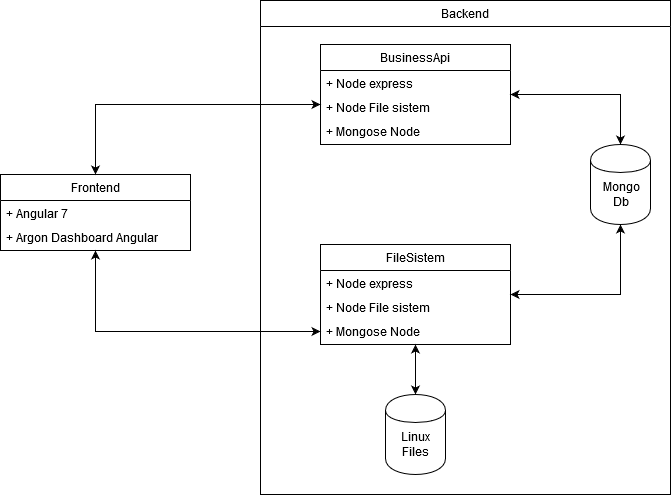
\includegraphics[width=430px,height=220px]{graphics/webArchitecture.PNG} \\
	\textbf{Fuente:} Elaborado por el autor de tesis
\end{figure}
\begin{itemize}
\item Front-end
	\begin{itemize}
	\item \textbf{Web}: Interfaz agradable para el usuario, cuya finalidad es realizar llamadas a las aplicaciones de negocio y servidor de archivos.
	\end{itemize}
\item Back-end
	\begin{itemize}
	\item \textbf{Business Api:} Maneja todas funciones l\'ogica del giro de negocios -e.g. Insertar movimiento, Leer movimiento, Resultados de rutina-.
	\item \textbf{File Sistem:} Interfaz de programaci\'on de aplicaciones que se encarga de almacenar los archivos metadata que define una base de datos del movimiento.
		\item \textbf{Linux Files:} Servidor encargado de almacenar los archivos de bases de datos del movimiento.
		\item \textbf{Mongo DB:} Servidor de bases de datos no relacional, que se encarga de almacenar informaci\'on respectiva del movimiento
	\end{itemize}
\item Entornos de trabajo
\begin{itemize}
\item \textbf{Angular 7:} Framework que facilita la creaci\'on y el mantenimiento de una aplicaci\'on web \cite{angular2019}.
\item \textbf{Argon Dashboard Angular:} Framework que facilita realizar una aplicaci\'on responsive -i.e. Adaptable a cualquier dispositivo a partir del navegador- \cite{argonDash}.
\item \textbf{Express js:} Framework encargado de realizar la comunicaci\'on entre aplicaciones, a partir del \acrlong{HTTP} \cite{fileSistem2019}.
\item \textbf{Mongoose:} Framework encargado de realizar cualquier operaci\'on de la base de datos de Mongo -e.g. Conexi\'on, recuperar datos, modificar- \cite{mongoose2019}.
\end{itemize}
\end{itemize}
As\'i mismo la aplicaci\'on web esta conformado por las siguientes 4 Vistas:
\paragraph{Vista del listado de movimientos}\mbox{} \\ \label{ins:UI:web:index}
Vista principal que muestra al usuario todos los movimientos que se han insertado en la base de datos.
\begin{figure}[H]
	\caption{Vista de Index de movimientos}
	\label{fig:viewIndex}
	\centering
	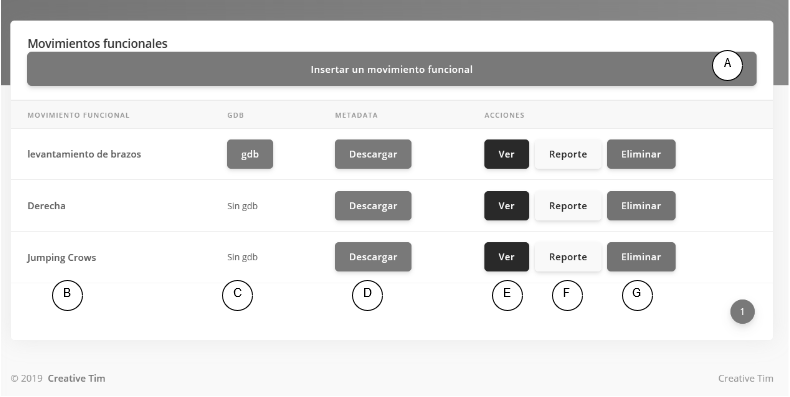
\includegraphics[width=440px,height=270px]{graphics/web-index.PNG} \\
	\textbf{Fuente:} Elaborado por el autor de tesis
\end{figure}
\begin{enumerate}[A.]
\item Bot\'on que dirige al usuario a la pantalla de insertar un movimiento (Ver vista \ref{ins:UI:web}.\ref{ins:UI:web:create}).
\item Etiqueta que indica el nombre del movimiento.
\item Bot\'on que descarga el archivo de base de datos de un movimiento.
\item Bot\'on que exporta el archivo de metadata de un movimiento (Ver anexos, c\'odigo \ref{code:jsonMeta}), con los siguientes atributos:
	\begin{itemize}
	\item \textbf{Steps}: Vector n\'umerico que contiene las etiquetas de cada paso de un movimiento.
	\item \textbf{anglesOfMovement}: Vector n\'umerico que almacena los \'indices de cada articulaci\'on que interact\'ua en el movimiento.
	\item \textbf{recognition}: Valor que construye  el rango de confiabilidad para detectar un paso de un movimiento.
	\item \textbf{id}: c\'odigo \'unico que identifica el movimiento en la base de datos.
	\item \textbf{height}: Altura del kinect con respecto al suelo (Medida en metros).	
	\item \textbf{depthMin}: Distancia m\'inima de profundidad del sensor y el atleta (Medida en metros).
	\item \textbf{depthMax}: Distancia m\'axima de profundidad del sensor y el atleta (Medida en metros).
	\item \textbf{timestamp}: Fecha en la cual fue insertado el registro del movimiento.
	\item \textbf{focusJoin}: Articulaci\'on de an\'alisis que permite medir la distancia de profundidad. 
	\end{itemize}
\item Bot\'on que dirige al usuario a la pantalla de detalle de un movimiento (Ver vista \ref{ins:UI:web}.\ref{ins:UI:web:read}).
\item Bot\'on que dirige al usuario a la pantalla de reporte de un movimiento (Ver vista \ref{ins:UI:web}.\ref{ins:UI:web:result}).
\item Bot\'on que elimina el registro del movimiento de la base de datos.
\end{enumerate}
\paragraph{Vista de creaci\'on de un movimiento}\mbox{} \\ \label{ins:UI:web:create}
Vista que se encarga de insertar toda la informaci\'on del movimiento, recuperada por los formularios.
\begin{figure}[H]
	\caption{Vista de crear un movimiento}
	\label{fig:viewCreate}
	\centering
	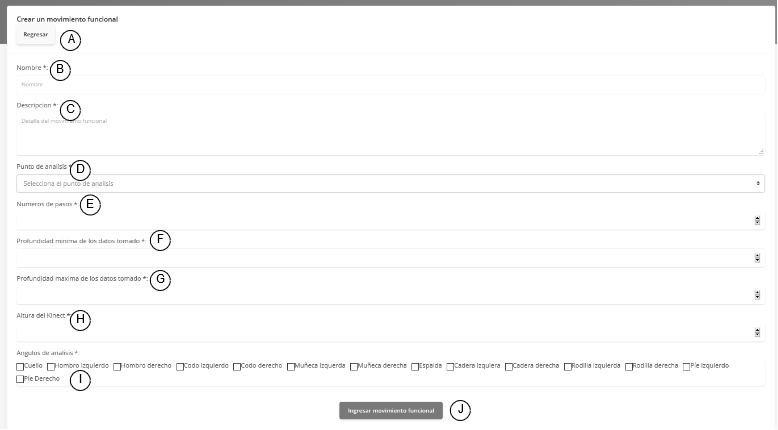
\includegraphics[width=460px,height=320px]{graphics/web-create.PNG} \\
	\textbf{Fuente:} Elaborado por el autor de tesis
\end{figure}
\begin{enumerate}[A.]
\item Bot\'on que dirige al usuario a la pantalla del listado de los movimientos (Ver vista \ref{ins:UI:web}.\ref{ins:UI:web:index}).
\item Textbox para ingresar el nombre del movimiento (Recuperado del formulario \ref{ins:frmMov}, atributo de nombre).
\item Textbox para ingresar el detalle del movimiento (Recuperado del formulario \ref{ins:frmMov}, atributo de descripci\'on).
\item Selecci\'on de la articulaci\'on de \'analisis (recuperado del formulario  \ref{ins:frmRout}, atributo de articulaci\'on de \'analisis).
\item Textbox n\'umerico que ingresa la cantidad de pasos del movimiento (recuperado del formulario  \ref{ins:frmMov}, atributo de n\'umero de pasos).
\item Textbox n\'umerico que ingresa la distancia m\'inima de profundidad (ver formula \ref{frm:maxDepth}).
\item Textbox n\'umerico que ingresa la distancia m\'axima de profundidad (ver formula \ref{frm:minDepth}).
\item Textbox n\'umerico que ingresa la altura del Kinect con respecto al suelo (Para el presente proyecto es de 0.70 metros, debido que es la altura de la mesa que daba soporte al sensor, ver secci\'on \ref{ins}).
\item Listado m\'ultiples de articulaciones que interviene en el movimiento (recuperado del formulario  \ref{ins:frmRout}, atributo de articulaciones no ignoradas).
\item Bot\'on que almacena toda la informaci\'on respectiva del formulario web.
\end{enumerate}
\paragraph{Vista de lectura de un movimiento}\mbox{} \\ \label{ins:UI:web:read}
Vista que se encarga de mostrar toda la informaci\'on del movimiento, adem\'as de insertar el archivo de base de datos de gesturas y modificar el rango de confiabilidad de reconocimiento de pasos.
\begin{figure}[H]
	\caption{Vista de lectura del movimiento}
	\label{fig:viewRead}
	\centering
	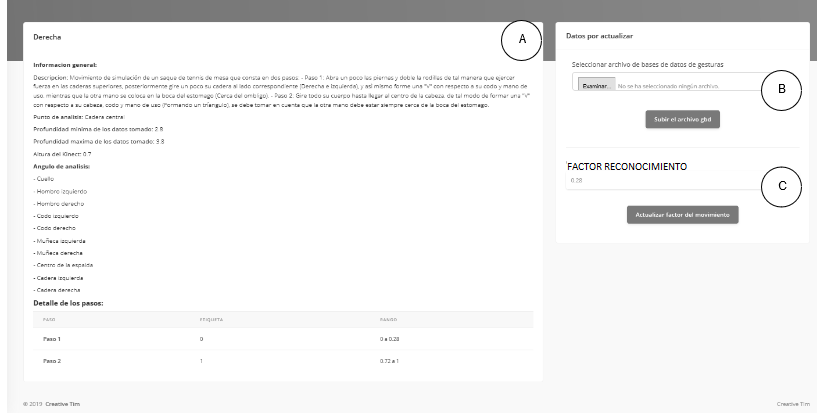
\includegraphics[width=460px,height=320px]{graphics/web-read.PNG} \\
	\textbf{Fuente:} Elaborado por el autor de tesis
\end{figure}
\paragraph{Vista de resultados de un movimiento}\mbox{} \\ \label{ins:UI:web:result}
Vista que expone los resultados de la aplicaci\'on de evaluaci\'on de un movimiento (Ver instrumento \ref{ins:UI:wpf}.\ref{ins:UI:wpf:evaluate})
\begin{figure}[H]
	\caption{Resultados de la rutina tabata de un movimiento}
	\label{fig:resultsTabata}
	\centering
	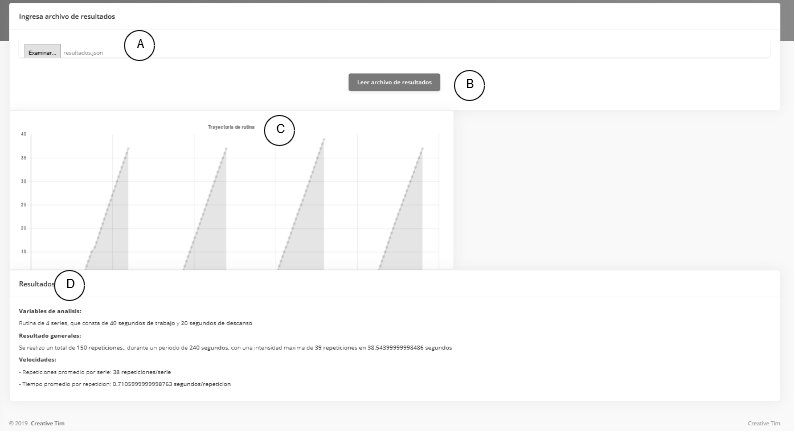
\includegraphics[width=460px,height=320px]{graphics/web-results.PNG} \\
	\textbf{Fuente:} Elaborado por el autor de tesis
\end{figure}

\subsubsection{Consola (Windows)}\mbox{} \\ \label{ins:cons} 

\subsection{Herramienta para el an\'alisis de datos} \label{ins:toolsAn}
Se utiliz\'o el software, Microsoft Excel, para la tabulaci\'on y organizaci\'on de los datos.